\documentclass[a4paper,12pt]{article}

% Packages usuels et encodage
\usepackage[utf8]{inputenc}
\usepackage[T1]{fontenc}
\usepackage[french, provide=*]{babel}
\usepackage{graphicx}
\usepackage{geometry}
\usepackage{hyperref}
\usepackage{listings}
\usepackage{xcolor}
\usepackage{float}
\usepackage{booktabs} % Pour de jolis tableaux
\usepackage{pgfplots}
\usepackage{tikz}
\usetikzlibrary{shapes.geometric, arrows, positioning, calc}
\pgfplotsset{compat=1.17}

% Configuration de la mise en page
\geometry{hmargin=2.5cm,vmargin=2.5cm}

% Configuration pour l'insertion de code (C/C++)
\definecolor{codegreen}{rgb}{0,0.6,0}
\definecolor{codegray}{rgb}{0.5,0.5,0.5}
\definecolor{codepurple}{rgb}{0.58,0,0.82}
\definecolor{backcolour}{rgb}{0.95,0.95,0.92}

\lstdefinestyle{mystyle}{
    backgroundcolor=\color{backcolour},   
    commentstyle=\color{codegreen},
    keywordstyle=\color{magenta},
    numberstyle=\tiny\color{codegray},
    stringstyle=\color{codepurple},
    basicstyle=\ttfamily\footnotesize,
    breakatwhitespace=false,         
    breaklines=true,                 
    captionpos=b,                    
    keepspaces=true,                 
    numbers=left,                    
    numbersep=5pt,                  
    showspaces=false,                
    showstringspaces=false,
    showtabs=false,                  
    tabsize=2,
    language=C++
}
\lstset{style=mystyle}

\title{Compte Rendu : Implémentation du Game of Life en CUDA}
\author{Hugo}
\date{8 Février 2026}

\begin{document}

\maketitle

\section{Introduction}
Ce document présente l'implémentation du noyau CUDA pour le Jeu de la Vie et les optimisations testées.

\section{Validation et Configuration}
L'exactitude de l'implémentation a été vérifiée en comparant les résultats du GPU avec une implémentation de référence en PyTorch. L'exécution de la commande suivante confirme la correspondance des résultats :
\begin{verbatim}
python conway.py test
> Both implementations match
\end{verbatim}

La configuration matérielle utilisée pour les tests est la suivante :
\begin{verbatim}
NVIDIA-SMI 535.288.01 Driver Version: 535.288.01 CUDA Version: 12.2
GPU: NVIDIA GeForce GTX 1070 (8192MiB)
\end{verbatim}

\section{Performances et Optimisations}
Une optimisation préliminaire a consisté à utiliser le type \texttt{unsigned char} (1 octet) au lieu de \texttt{int} (4 octets) pour stocker les états des cellules. Cette modification permet de diviser par quatre l'empreinte mémoire de la grille et d'optimiser l'utilisation de la bande passante mémoire ainsi que du cache.

L'implémentation actuelle utilise également des \textbf{grid-stride loops} pour permettre au noyau de traiter des grilles de n'importe quelle taille, indépendamment de la taille de la grille de blocs CUDA. Cela améliore la robustesse et permet une meilleure réutilisation des threads.

Plusieurs versions du noyau ont été testées pour l'application des règles du Jeu de la Vie.

\subsection{Version 1 : Expression Booléenne Directe}
Cette version utilise une expression logique concise pour déterminer l'état suivant :
\begin{lstlisting}[language=C++]
new_grid[idx] = alive_neighbors == 3 || (grid[idx] == 1 && alive_neighbors == 2);
\end{lstlisting}
Performance obtenue : \textbf{1001 FPS}.

\subsection{Version 2 : Branchements Conditionnels}
Cette version utilise des structures \texttt{if/else} plus explicites (bien que logiquement redondantes dans ce cas précis) :
\begin{lstlisting}[language=C++]
new_grid[idx] = 0;
if (grid[idx] == 0 && alive_neighbors == 3 || 
    (grid[idx] == 1 && (alive_neighbors == 4 || alive_neighbors == 3))) {
    new_grid[idx] = 1;
}
else if (grid[idx] == 1 && (alive_neighbors == 4 || alive_neighbors == 3)) {
    new_grid[idx] = 1;
}
\end{lstlisting}
Performance obtenue : \textbf{1057.26 FPS}.

\subsection{Version 3 : Mémoire Partagée (Shared Memory)}
L'optimisation repose sur l'utilisation de la \textit{Shared Memory}. L'idée est de réduire les accès à la mémoire globale lente en chargeant une tuile de données dans une mémoire locale rapide partagée par les threads d'un même bloc.

\begin{figure}[H]
    \centering
    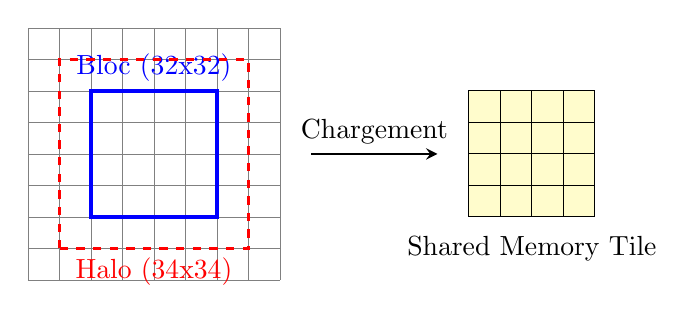
\begin{tikzpicture}[scale=0.8]
        % Grille Globale
        \draw[step=0.5cm,gray,very thin] (0,0) grid (4,4);
        \draw[line width=1.5pt, blue] (1,1) rectangle (3,3);
        \node[blue, above] at (2,3) {Bloc (32x32)};
        
        % Halo
        \draw[line width=1pt, red, dashed] (0.5,0.5) rectangle (3.5,3.5);
        \node[red, below] at (2,0.5) {Halo (34x34)};
        
        % Annotation
        \draw[->, >=stealth, thick] (4.5,2) -- (6.5,2) node[midway, above] {Chargement};
        
        % Shared Memory
        \begin{scope}[shift={(7,1)}]
            \draw[fill=yellow!20] (0,0) rectangle (2,2);
            \draw[step=0.5cm, black, thin] (0,0) grid (2,2);
            \node at (1,-0.5) {Shared Memory Tile};
        \end{scope}
    \end{tikzpicture}
    \caption{Schéma du chargement de la tuile et du halo en mémoire partagée.}
\end{figure}

Chaque bloc de 32x32 threads charge une zone de 34x34 (\textit{halo} de 1 pixel) pour permettre le calcul des voisins sur les bords sans accès mémoire globale supplémentaire.

L'implémentation du noyau utilisant la mémoire partagée est la suivante :

\begin{lstlisting}[language=C++]
__global__ void game_of_life_kernel(unsigned char *grid, unsigned char *new_grid, int width, int height) {
    __shared__ unsigned char tile[34][34];
    int tx = threadIdx.x; int ty = threadIdx.y;
    int x = blockIdx.x * 32 + tx; int y = blockIdx.y * 32 + ty;

    // Chargement collaboratif avec halo
    int tid = ty * 32 + tx;
    int block_start_x = blockIdx.x * 32 - 1;
    int block_start_y = blockIdx.y * 32 - 1;

    for (int i = tid; i < 34 * 34; i += 1024) {
        int ly = i / 34; int lx = i % 34;
        int gx = block_start_x + lx; int gy = block_start_y + ly;
        unsigned char val = 0;
        if (gx >= 0 && gx < width && gy >= 0 && gy < height)
            val = grid[gy * width + gx];
        tile[ly][lx] = val;
    }
    __syncthreads();

    if (x < width && y < height) {
        int sx = tx + 1; int sy = ty + 1;
        int neighbors = tile[sy-1][sx-1] + tile[sy-1][sx] + tile[sy-1][sx+1] +
                        tile[sy][sx-1]   +                  tile[sy][sx+1] +
                        tile[sy+1][sx-1] + tile[sy+1][sx] + tile[sy+1][sx+1];
        unsigned char current = tile[sy][sx];
        new_grid[y * width + x] = (neighbors == 3) | (current & (neighbors == 2));
    }
}
\end{lstlisting}

Performance obtenue : \textbf{1165.18 FPS}.

\subsection{Version 4 : Lookup Table (LUT) et Vectorisation}
Pour cette version, nous changeons de paradigme. Au lieu de calculer l'état futur cellule par cellule, nous utilisons une table de correspondance (Lookup Table) précalculée.

L'idée est qu'un bloc de $2 \times 2$ cellules (4 pixels) dépend entièrement de l'état d'un bloc de $4 \times 4$ cellules qui l'entoure.
Un bloc de $4 \times 4$ contient 16 cellules, ce qui correspond exactement à un entier de 16 bits ($2^{16} = 65536$ possibilités).

\begin{figure}[H]
    \centering
    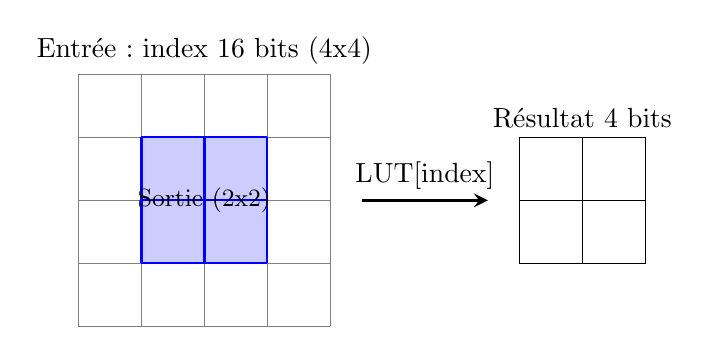
\begin{tikzpicture}[scale=0.8]
        % Grille 4x4
        \draw[step=1cm, gray, thin] (0,0) grid (4,4);
        \node[above] at (2,4) {Entrée : index 16 bits (4x4)};
        
        % Cellules centrales 2x2
        \fill[blue!20] (1,1) rectangle (3,3);
        \draw[step=1cm, blue, thick] (1,1) grid (3,3);
        \node at (2,2) { \small Sortie (2x2)};
        
        % Flèche vers LUT
        \draw[->, >=stealth, very thick] (4.5, 2) -- (6.5, 2) node[midway, above] {LUT[index]};
        
        % Résultat
        \draw (7, 1) rectangle (9, 3);
        \draw[step=1cm, black] (7,1) grid (9,3);
        \node[above] at (8,3) {Résultat 4 bits};
    \end{tikzpicture}
    \caption{Principe de la LUT : Un voisinage 4x4 détermine le futur des 4 cellules centrales.}
\end{figure}

Nous précalculons donc une table de 65536 entrées en mémoire globale. Chaque entrée contient les 4 bits de résultat pour le bloc central.

Le noyau CUDA est modifié pour que **chaque thread traite désormais 4 pixels** (un bloc $2 \times 2$). Le nombre de threads est donc divisé par 4, réduisant le surcoût de lancement et augmentant l'intensité arithmétique (ici remplacée par des opérations sur les bits).

\begin{lstlisting}[language=C++]
// Extrait du kernel
int tile_r = 2 * ty;
int tile_c = 2 * tx;
uint16_t state_idx = 0;

// Construction de l'index 16 bits depuis la shared memory
#pragma unroll
for (int r = 0; r < 4; r++) {
    for (int c = 0; c < 4; c++) {
        if (tile[tile_r + r][tile_c + c]) {
            state_idx |= (1 << (r * 4 + c));
        }
    }
}

// Lecture unique en memoire pour 4 pixels
unsigned char res = lut[state_idx];

// Ecriture des 4 pixels
new_grid[...] = (res >> 0) & 1;
new_grid[...] = (res >> 1) & 1;
// ... (idem pour les 2 autres)
\end{lstlisting}

Performance obtenue : \textbf{2455.34 FPS}.
C'est un gain considérable (\textbf{+110\%} par rapport à la version shared memory) qui s'explique par la vectorisation du travail (1 thread = 4 pixels) et la suppression complète des branchements et des calculs arithmétiques au profit d'opérations bit-à-bit très rapides.

\section{Analyse}
De manière surprenante, la version avec branchements (Version 2) affiche une performance légèrement supérieure à la version booléenne compacte. 
Cependant, l'introduction de la \textbf{Shared Memory} (Version 3) a apporté un premier gain important. 
Enfin, l'approche \textbf{Lookup Table} (Version 4) écrase les précédentes en transformant le problème de calcul en un problème d'accès mémoire optimisé et vectorisé.

\subsection{Version 5 : Maximisation de l'Occupation (1024 Threads)}
L'optimisation précédente utilisait des blocs de $16 \times 16$ threads (256 threads) couvrant une zone de $32 \times 32$ pixels.
Cependant, les GPU modernes supportent jusqu'à 1024 threads par bloc.

Nous avons donc augmenté la taille des blocs à $32 \times 32$ threads (1024 threads). Comme chaque thread traite toujours un carré de $2 \times 2$ pixels, chaque bloc CUDA couvre désormais une zone de $64 \times 64$ pixels sur la grille.

\textbf{Avantages :}
\begin{itemize}
    \item Meilleure occupation du multiprocesseur (SM).
    \item Réduction du ratio \textit{Halo / Données utiles}. Pour une tuile de $32^2$ pixels, le halo est de $34^2 - 32^2 = 132$ pixels. Pour $64^2$ pixels, le halo est de $66^2 - 64^2 = 260$ pixels. Le ratio halo/pixels passe de $132/1024 \approx 12.8\%$ à $260/4096 \approx 6.3\%$.
\end{itemize}

Résumé des performances :
\begin{center}
\begin{tabular}{lc}
\toprule
Version & FPS \\
\midrule
Naive (Booléenne) & 1001.00 \\
Naive (Branchements) & 1057.26 \\
Shared Memory & 1165.18 \\
Lookup Table (256 threads) & 2455.34 \\
\textbf{Lookup Table (1024 threads)} & \textbf{--} \\
\bottomrule
\end{tabular}
\end{center}

\newpage
\section{Version Finale : Bit-Patching et Registres 64-bits}

Dans cette version, on exploite les registres 64 bits du GPU.
Chaque thread est responsable d'un entier \texttt{uint16\_t}, qui représente un bloc de $4 \times 4$ cellules.

\begin{figure}[H]
    \centering
    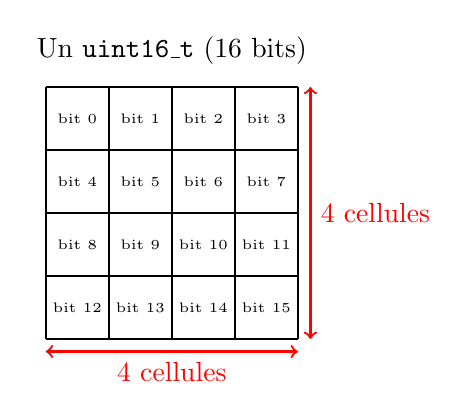
\begin{tikzpicture}[scale=0.8]
        \draw[step=1cm, black, thick] (0,0) grid (4,4);
        \node[above] at (2,4.2) {Un \texttt{uint16\_t} (16 bits)};
        \foreach \y in {0,1,2,3} {
            \foreach \x in {0,1,2,3} {
                \pgfmathsetmacro{\idx}{int((3-\y)*4 + \x)}
                \node at (\x+0.5, \y+0.5) {\tiny bit \idx};
            }
        }
        \draw[<->, red, thick] (4.2,0) -- (4.2,4) node[midway, right] {4 cellules};
        \draw[<->, red, thick] (0,-0.2) -- (4,-0.2) node[midway, below] {4 cellules};
    \end{tikzpicture}
    \caption{Représentation compacte : 16 cellules stockées dans un seul registre.}
\end{figure}

\subsection{Le Problème du Voisinage}
Pour calculer l'état futur de notre bloc $4 \times 4$ (Centre), nous avons besoin de connaître l'état de ses voisins immédiats (cellules bordures). Ce voisinage forme une grille de $6 \times 6$ cellules.

Les données nécessaires proviennent de **9 blocs** \texttt{uint16\_t} différents : le bloc central et ses 8 voisins (Nord, Sud, Est, Ouest, et les diagonales).

\subsection{L'Algorithme de "Super-Patch" 64 bits}
Au lieu d'aller chercher les valeurs en mémoire à chaque calcul, nous construisons un objet virtuel temporaire dans les registres du thread : le **Patch**.

Un carré de $6 \times 6$ cellules correspond à 36 bits.
Comme $36 < 64$, nous pouvons stocker l'intégralité du voisinage nécessaire dans un seul registre \texttt{uint64\_t}.

\begin{figure}[H]
    \centering
    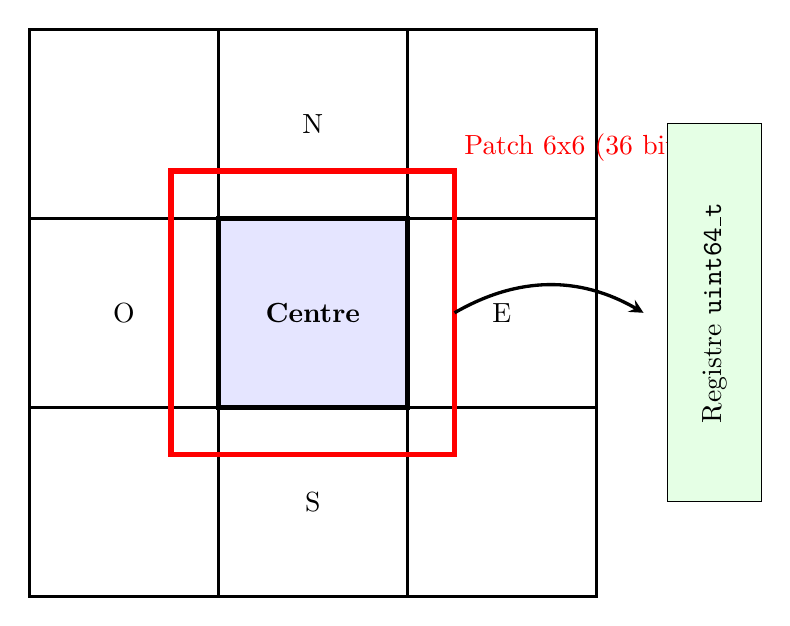
\begin{tikzpicture}[scale=0.6]
        % Voisinage 3x3 blocs
        \foreach \i in {0,1,2} {
            \foreach \j in {0,1,2} {
                \draw[gray, thin] (\i*4, \j*4) rectangle (\i*4+4, \j*4+4);
            }
        }
        % Thicker separators between uint16 blocks (every 4 cells)
        \draw[line width=1.2pt, black] (0,0) rectangle (12,12);
        \draw[line width=1pt, black] (4,0) -- (4,12); \draw[line width=1pt, black] (8,0) -- (8,12);
        \draw[line width=1pt, black] (0,4) -- (12,4); \draw[line width=1pt, black] (0,8) -- (12,8);

        % Centre (highlighted) - thicker border for clarity
        \draw[fill=blue!10, line width=2pt] (4,4) rectangle (8,8);
        \node at (6,6) {\textbf{Centre}};
        \node at (6,10) {N}; \node at (10,6) {E}; \node at (2,6) {O}; \node at (6,2) {S};
        
        % Zone utile (Patch 6x6)
        \draw[red, line width=2pt] (3,3) rectangle (9,9);
        \node[red, above right] at (9,9) {Patch 6x6 (36 bits)};
        
        % Flèche vers le registre
        \draw[->, >=stealth, very thick, bend left] (9,6) to (13,6);
        
        % Registre 64 bits
        \draw[fill=green!10] (13.5, 2) rectangle (15.5, 10);
        \node[rotate=90] at (14.5, 6) {Registre \texttt{uint64\_t}};
        
    \end{tikzpicture}
    \caption{Construction du Patch : on extrait les bits nécessaires des 9 voisins pour former un seul mot de 64 bits.}
\end{figure}

Une fois ce \texttt{uint64\_t patch} construit via des opérations bit-à-bit (masques et décalages), le thread n'a plus besoin d'accéder à la mémoire. Il contient toute l'information localement.

% ------------------ Schéma détaillé (6x6) ------------------
\begin{figure}[H]
    \centering
    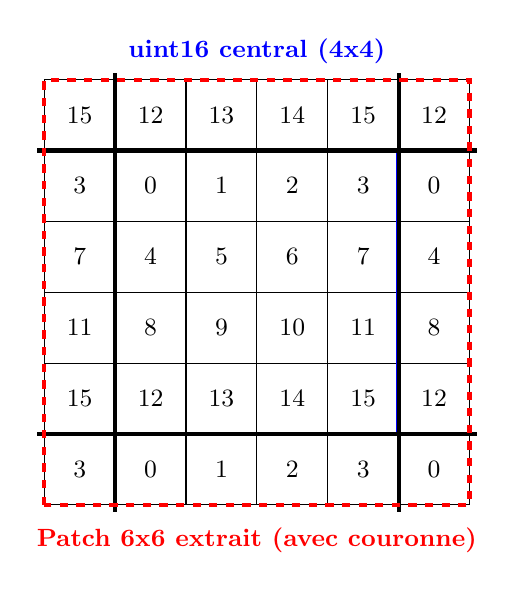
\begin{tikzpicture}[scale=0.9, every node/.style={font=\small, minimum size=6mm}]
        % Draw 6x6 cells with numbers
        \foreach \r in {0,...,5} {
            \foreach \c in {0,...,5} {
                \draw (\c,5-\r) rectangle (\c+1,5-\r+1);
            }
        }
        % Fill numbers matching the requested layout (top to bottom)
        % Row 0 (top): 15 12 13 14 15 12
        \node at (0.5,5.5) {15}; \node at (1.5,5.5) {12}; \node at (2.5,5.5) {13}; \node at (3.5,5.5) {14}; \node at (4.5,5.5) {15}; \node at (5.5,5.5) {12};
        % Row 1: 3 0 1 2 3 0
        \node at (0.5,4.5) {3};  \node at (1.5,4.5) {0};  \node at (2.5,4.5) {1};  \node at (3.5,4.5) {2};  \node at (4.5,4.5) {3};  \node at (5.5,4.5) {0};
        % Row 2: 7 4 5 6 7 4
        \node at (0.5,3.5) {7};  \node at (1.5,3.5) {4};  \node at (2.5,3.5) {5};  \node at (3.5,3.5) {6};  \node at (4.5,3.5) {7};  \node at (5.5,3.5) {4};
        % Row 3: 11 8 9 10 11 8
        \node at (0.5,2.5) {11}; \node at (1.5,2.5) {8};  \node at (2.5,2.5) {9};  \node at (3.5,2.5) {10}; \node at (4.5,2.5) {11}; \node at (5.5,2.5) {8};
        % Row 4: 15 12 13 14 15 12
        \node at (0.5,1.5) {15}; \node at (1.5,1.5) {12}; \node at (2.5,1.5) {13}; \node at (3.5,1.5) {14}; \node at (4.5,1.5) {15}; \node at (5.5,1.5) {12};
        % Row 5: 3 0 1 2 3 0
        \node at (0.5,0.5) {3};  \node at (1.5,0.5) {0};  \node at (2.5,0.5) {1};  \node at (3.5,0.5) {2};  \node at (4.5,0.5) {3};  \node at (5.5,0.5) {0};

        % Highlight central 4x4 (the uint16 central)
        \draw[line width=1.7pt, blue] (1,1) rectangle (5,5);
        \node[blue] at (3,6.4) {\textbf{uint16 central (4x4)}};

        % Emphasize uint16 block boundaries (every 4 cells) around the center
        % \draw[line width=1.2pt, black] (-0.1,-0.1) rectangle (6.1,6.1);
        \draw[line width=1.5pt, black] (1, -0.1) -- (1, 6.1); \draw[line width=1.5pt, black] (5, -0.1) -- (5, 6.1);
        \draw[line width=1.5pt, black] (-0.1,1) -- (6.1,1); \draw[line width=1.5pt, black] (-0.1,5) -- (6.1,5);

        % Highlight extracted 6x6 area
        \draw[line width=1.5pt, red, dashed] (0,0) rectangle (6,6);
        \node[red] at (3, -0.5) {\textbf{Patch 6x6 extrait (avec couronne)}};
    \end{tikzpicture}
    \caption{Numérotation des bits dans le bloc central 4x4 et la couronne 6x6 extraite par \texttt{build\_patch6x6}.}
\end{figure}

\paragraph{Explication détaillée du code}
Le code effectue pour chaque ligne i de 0 à 5 :
\begin{itemize}
    \item i == 0 : on construit la ligne au-dessus (row r-1) à partir des dernières lignes des blocs NO, N, NE. \texttt{mid4 = (N >> 12) \& 0xF} lit la dernière ligne du bloc N; \texttt{left\_bit = (NO >> 15) \& 1} lit le bit le plus à droite (col 3) de la dernière ligne de NO; \texttt{right\_bit = (NE >> 12) \& 1} lit le bit le plus à gauche (col 0) de la dernière ligne de NE.
    \item i == 1..4 : pour chaque ligne du centre on lit la ligne correspondante de \texttt{C} via \texttt{mid4 = (C >> (4*ri)) \& 0xF} (ri = i-1), et on récupère la colonne de gauche depuis \texttt{O} et la colonne de droite depuis \texttt{E} (bits isolés par des shifts appropriés).
    \item i == 5 : on construit la ligne sous le centre (row r+4) à partir des premières lignes de SO, S, SE (ex. \texttt{mid4 = (S >> 0) \& 0xF}).
\end{itemize}

Ces 6 lignes de 6 bits sont concaténées (\texttt{patch |= (uint64\_t)row6 << (6 * i)}) pour former le mot 36 bits logé dans un \texttt{uint64\_t}. Ensuite on extrait des fenêtres 4x4 par décalages successifs pour indexer la LUT.

\subsection{Extraction et Lookup par Quadrants}
Nous divisons ensuite notre problème $4 \times 4$ en quatre sous-problèmes $2 \times 2$ (quadrants).
Pour chaque quadrant, nous extrayons une fenêtre de $4 \times 4$ bits depuis le patch 64 bits, ce qui nous donne un index pour interroger la LUT.

\begin{lstlisting}[language=C++]
// Exemple conceptuel
uint64_t patch = build_patch6x6(N, S, E, O, ...);

// On extrait 4 fenetres depuis le patch
uint16_t idx_TL = extract(patch, 0, 0); // Top-Left
uint16_t idx_TR = extract(patch, 0, 2); // Top-Right
uint16_t idx_BL = extract(patch, 2, 0); // Bot-Left
uint16_t idx_BR = extract(patch, 2, 2); // Bot-Right

// Lookup instantanee
uint8_t res_TL = lut[idx_TL];
uint8_t res_TR = lut[idx_TR];
...

// Assemblage final
uint16_t result = (res_TL) | (res_TR << 2) | ...;
\end{lstlisting}

\subsection{Avantages de cette méthode}
\begin{enumerate}
    \item \textbf{Réduction drastique des accès mémoire :} Une fois les blocs chargés en \textit{Shared Memory}, tout le calcul se fait dans les registres.
    \item \textbf{Zéro divergence :} Tous les threads exécutent exactement les mêmes opérations binaires, il n'y a aucun \texttt{if/else}.
    \item \textbf{Parallélisme de bits :} En manipulant des \texttt{uint16} et \texttt{uint64}, nous traitons 16 cellules simultanément par thread avec un nombre d'instructions très faible.
\end{enumerate}

Cette implémentation représente l'état de l'art pour les automates cellulaires sur GPU, transformant un problème de calcul arithmétique en un problème de pure manipulation de bits.

\end{document}
